
% *********** chapter0.tex
\chapter{Introduction}
\label{ch:cad-intro}
\section{Implicit form}

Among the different representations to describe a quarter of circle (of radius $1$ and centered at the origin), one can use an implicit form using the equation
\begin{align*}
  f(x,y) := x^2 + y^2 - 1 = 0, \quad x \ge 0 ~ \mbox{and} ~ y \ge 0 
\end{align*}
\noindent
In practice, implicit forms are well adapted for unbounded geometries. On the other hand, given a point, it is easy to determine if it is on the curve or a surface. Although, this is an important question, in general, we are interested in geometric manipulations in CAD systems, such as improving the resolution, smoothness and having local control of a given curve or surface. These properties are very difficult to ensure when using an implicit form; at the end, a computer needs discrete values in order to plot or manipulate a CAD object, which is in opposition with the analytical form represented by an equation. 


\section{Parametric curves}
Another way of representing a quarter of circle is to consider the parametric curve define in \ref{eq:quarter-circle-polair}, where $\theta \in \left[ 0, \frac{\pi}{2} \right]$
\begin{align}
  \mathcal{C}(\theta) = 
  \begin{bmatrix}
    x(\theta) \\ y(\theta)
  \end{bmatrix} =
  \begin{bmatrix}
    \cos \theta \\ \sin \theta
  \end{bmatrix}
  \label{eq:quarter-circle-polair}
\end{align}
\begin{figure}
\centering
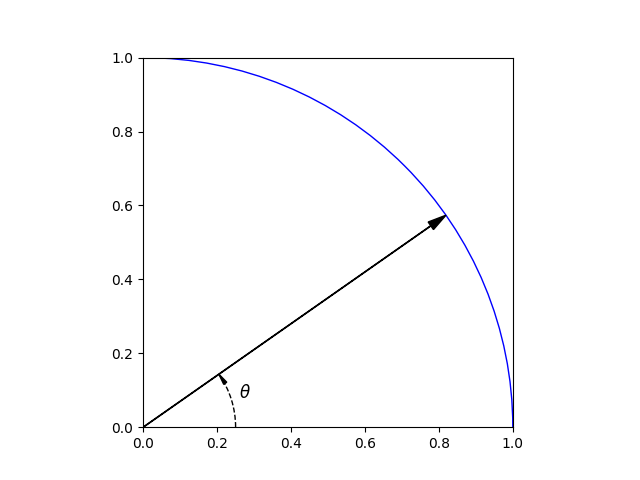
\includegraphics[width=0.6\textwidth]{figures/cad/quarter_circle_polar}
\caption{Quarter of circle of radius 1, using polar coordinates.}
\label{fig:quarter_circle_polar}
\end{figure}

in which case we can compute its derivative as 
\begin{align}
  \mathcal{C}^\prime(\theta) = 
  \begin{bmatrix}
    -\sin \theta \\ \cos \theta
  \end{bmatrix}
  \label{eq:quarter-circle-polair-derivative}
\end{align}
The tangent at $\theta = 0$ and $\theta = \frac{\pi}{2}$ are then given by 
$\mathcal{C}^\prime(\theta := 0) = 
  \begin{bmatrix}
    0 \\ 1 
  \end{bmatrix}
$ 
and 
$\mathcal{C}^\prime(\theta := \frac{\pi}{2}) = 
  \begin{bmatrix}
    -1 \\ 0 
  \end{bmatrix}
$.
\\
\noindent
Another way to represent the quarter of circle, is to introduce the variable $t := \tan \frac{\theta}{2}$, then we get the following rational form \ref{eq:quarter-circle-rational}, where $t \in \left[ 0, 1 \right]$,
\begin{align}
  \mathcal{C}(t) = 
  \begin{bmatrix}
    x(t) \\ y(t)
  \end{bmatrix} =
  \begin{bmatrix}
    \frac{1-t^2}{1+t^2} \\ \frac{2t}{1+t^2}
  \end{bmatrix}
  \label{eq:quarter-circle-rational}
\end{align}

\noindent
There are different advantages for having a parametric form:
\begin{itemize}
  \item Extending a 2D curve to 3D,
  \item Ideal for bounded curves and surfaces,   
  \item Natural orientation of curves and surfaces,
  \item Appropriate representation for design on a computer. In some particular cases, the coefficients in a parametric form possess interesting geometric significance, 
  \item Computing a point on a curve is easy, while finding its parametric value is a in general a non-linear problem, 
\end{itemize}

\begin{remark}
  Notice that in some cases, this representation may introduce singularities that are unrelated to the described geometry.
\end{remark}

\begin{remark}
  Computing the derivatives (tangent or normal vectors at the extremeties) needs an evaluation. We shall be more interested in representation where such informations can be extracted directly from the parametric representations.
\end{remark}

Although one can use any parametric representation for CAD systems, it is important to restrict to a representation that is
\begin{itemize}
  \item capable of reproducing a \textit{wild class} of curves/surfaces
  \item easy to implement
  \item efficient and accurate evaluation 
  \item numerical stable evaluation
  \item \textit{easy} evaluation of points and their derivatives
  \item evaluation complexity of the same or comparable order as polynomials
  \item small memory storage
\end{itemize}

\section{Power basis form of a curve}
If we restrict our representation to polynomials, one naive way would be to use power basis, \textit{i.e.} monomials as in \ref{eq:power-basis-curve}
\begin{align}
  \mathcal{C}(t) = \sum_{i=0}^n \mathbf{a}_i t^i
  \label{eq:power-basis-curve}
\end{align}
where $\mathbf{a}_i = 
\begin{bmatrix}
  a_i^x \\ a_i^y \\ a_i^z
\end{bmatrix}
$ are 2D or 3D vectors.
\\
\noindent
Using the Taylor expansion, we get $\mathcal{C}^\prime(t)|_{t=0} = i! \mathbf{a}_i$, which leads to $\mathbf{a}_i = \frac{\mathcal{C}^\prime(t)|_{t=0}}{i!}$. We then have a direct access to the derivative at $t=0$, but only at this point.
\\
\noindent
The evaluation of such a form can be done using the Horner algorithm as described in \ref{eq:horner-algoritm}:

\begin{align}
  \mathcal{C}(t) = a_0 + t \left( a_1 + t \left( a_2 + t \left( \dots  + t \left( a_{n-1} + t a_{n}    \right)   \right) \right) \right) 
  \label{eq:horner-algoritm}
\end{align}

% ...
\begin{minipage}{\textwidth}
  \begin{algorithm}[H]
  \DontPrintSemicolon
  \SetAlgoLined
  \SetKwInOut{Input}{Input}\SetKwInOut{Output}{Output}
  \Input{$\mathbf{a}, x$}
  \Output{$v$}
  \BlankLine

  $n \gets {\sc len } \left( \mathbf{P} \right) - 1$\;
  $v \gets a[n]$\;
  \For{$i \gets n-1$ \textbf{to} $0$} {
    $v \gets v x + a[i]$\;
  }
  \Return{$v$}\;

  \caption{{\sc Horner}: Evaluation of a polynomial defined by its coefficients $\mathbf{a}$ at $x$.}
  \label{algo:horner}
  \end{algorithm} 
\end{minipage}
% ...

%The Python code \ref{code:horner}, implementations the sequential Horner algorithm.
%
%\begin{code}
%  \centering
%  \begin{python}
%  def horner(a, x):
%      """
%      evaluation of a power basis curve at a point 'x'.
%      'a' contains the coefficients
%      """
%      n = len(a) - 1
%      c = a[n]
%      for i in range(0, n)[::-1]:
%          c = c*x + a[i]
%      return c
%  \end{python}
%  \caption{Python implementation of the sequential Horner algorithm.}
%  \label{code:horner}
%\end{code}

\begin{remark}
  The Horner algorithm is numerically unstable for high degrees, more details can be found in  \cite{FAROUKI1987191} \cite{FAROUKI19881} \cite{HighamBook2002} \cite{Boldo2004}.
\end{remark}

%\todo{add example + exercise + check it using the Python code}

\begin{remark}
  The use of power basis form is not suited for shape and geometric design; the coefficients do not have any geoemtric meaning and modifying them do not allow for a good control of a curve or a surface,  
\end{remark}

% ...................................................................
\section{Problems}
\label{sec:cad-intro-problems}

\begin{exercise}
  Consider the two parametric representations of the circular arc given by Eqs. (\ref{eq:quarter-circle-polair}) and (\ref{eq:quarter-circle-rational}). Using Eq. (\ref{eq:quarter-circle-polair}), compute the curve point at $u = \frac{\pi}{4}$ and, using Eq. (\ref{eq:quarter-circle-rational}), the point at $t = \frac{1}{2}$. Explain the results.
\end{exercise}

\begin{exercise}
  Compute the acceleration vector, $\mathcal{C}^{\prime\prime}(u)$, for Eq. (\ref{eq:quarter-circle-polair}). Explain the result.
\end{exercise}

\begin{exercise}
  Consider the parabolic arc $\mathcal{C}^{\prime\prime}(u) = (x(u), y(u)) = \left( -1-u+2u^2, -2u, u^2 \right)$ for $0 \leq u \leq 1$. Plot the curve $\mathcal{C}$, then apply the transformations
  \begin{itemize}
    \item a rotation of $\frac{\pi}{2}$ about the origin. We recall that the rotation matrix (applied from the left) is 
      \begin{align*}
        \begin{pmatrix}
          0 & -1 \\
          1 &  0
        \end{pmatrix}
      \end{align*}
    \item a translation with the vector $\left( -1, -1 \right)$.
  \end{itemize}
  Compute the implicit equation of the associated parabola.
\end{exercise}

\begin{exercise}
  Determine formulas for the number of additions and multiplications necessary to compute a point on an nth-degree three-dimensional power basis curve.
\end{exercise}

\begin{exercise}
  Construct a cubic power basis curve with a loop. Hint: think about what end- points and end derivatives, $\mathcal{C}^\prime(0)$ and $\mathcal{C}^\prime(1)$, are necessary.
\end{exercise}

\begin{exercise}
Construct a cubic power basis curve with a cusp. Hint: think about $\mathcal{C}^\prime(u)$ and
$\mathcal{C}^{\prime\prime}(u)$. 
Sketch what $x^{\prime}(u), y^{\prime}(u), x^{\prime\prime}(u)$, and $y^{\prime\prime}(u)$ need to look like as functions of $u$.
Determine a suitable $\mathcal{C}^{\prime\prime}(u)$, and then integrate to obtain $\mathcal{C}^\prime(u)$ and $\mathcal{C}(u)$.
\end{exercise}

\begin{exercise}
Construct a cubic power basis curve with an inflection point.
\end{exercise}

\begin{exercise}
  Compare the CPU cost for an evaluation for the presented representations.
  % 60 + 60 for polar case
\end{exercise}

\begin{exercise}
  Compute the CPU cost for the Horner algorithm.
\end{exercise}

\begin{exercise}
  Write a Python implementation for the Horner algorithm.
\end{exercise}

\begin{exercise}[Parallel evaluation]
  Let us consider a polynomial $P$ of degree $n$, defined as $P(t) = \sum_{i=0}^{n} a_i t^i$. Using the form 
  \begin{align*}
   P(t) = \sum_{j=0}^{k-1} x^j P_j(x^k) 
  \end{align*}
  as a splitting into $k$ independent parts, write a Python code for the parallel evaluation and compute its complexity.
\end{exercise}


% *********** chapter1.tex
\chapter{B\'ezier curves}
%\minitoc
\label{ch:cad-bezier}
\section{Bernstein polynomials}
In 1885, Weierstrass proved that the set of polynomial functions on $\left[0, 1\right]$ is dense in $\mathcal{C}\left( \left[0, 1\right] \right)$. In 1912, Sergei Bernstein gave a simple proof to this result by introducing the now-famous Bernstein polynomials \ref{eq:bernstein}:

\begin{align}
  B_k^n (x) =  \binom{n}{k} x^k (1-x)^{n-k}, \quad \mbox{where}\quad k \in \left[0, n \right] ~ \mbox{and} ~ x \in \left[ 0, 1 \right]
  \label{eq:bernstein}
\end{align}
\noindent
In figure Fig. \ref{fig:bernstein}, we plot Bernstein polynomials of degrees $1$ to $5$. From these plots, we see that Bernstein polynomials are positive, the first and last polynomials are equal to $1$ on the $0$ and $1$ respectivaly. More properties will be discussed in the sequel.

%
\begin{figure}[ht!]
\centering
\begin{minipage}[t]{0.43\textwidth}
  \centering
  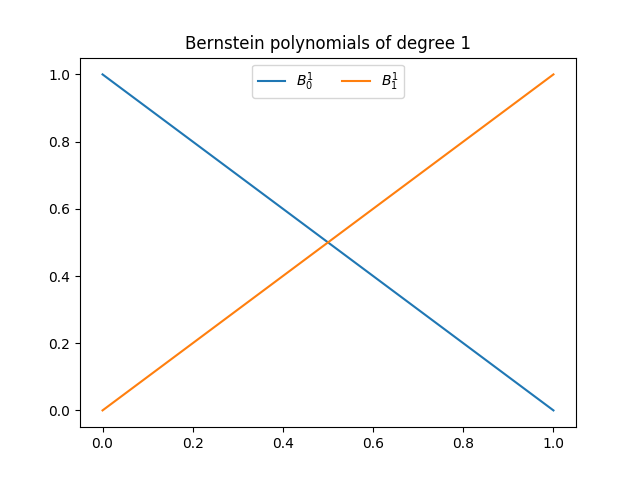
\includegraphics[width=1.0\textwidth]{figures/cad/all_bernstein_degree_1}
\end{minipage}
\begin{minipage}[t]{0.43\textwidth}
  \centering
  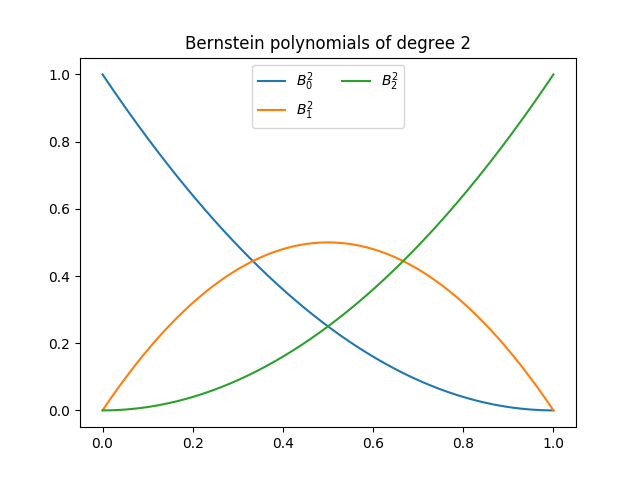
\includegraphics[width=1.0\textwidth]{figures/cad/all_bernstein_degree_2}
\end{minipage}
\begin{minipage}[t]{0.43\textwidth}
  \centering
  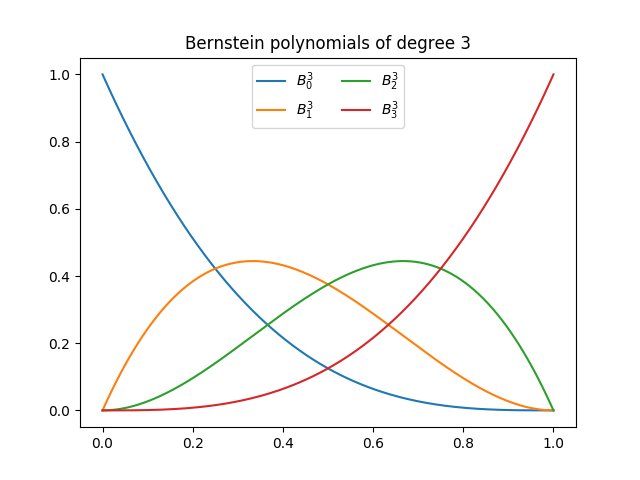
\includegraphics[width=1.0\textwidth]{figures/cad/all_bernstein_degree_3}
\end{minipage}
\begin{minipage}[t]{0.43\textwidth}
  \centering
  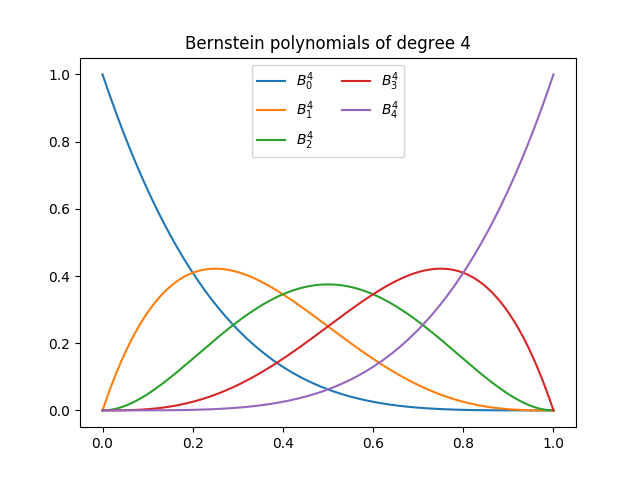
\includegraphics[width=1.0\textwidth]{figures/cad/all_bernstein_degree_4}
\end{minipage}
\begin{minipage}[t]{0.43\textwidth}
  \centering
  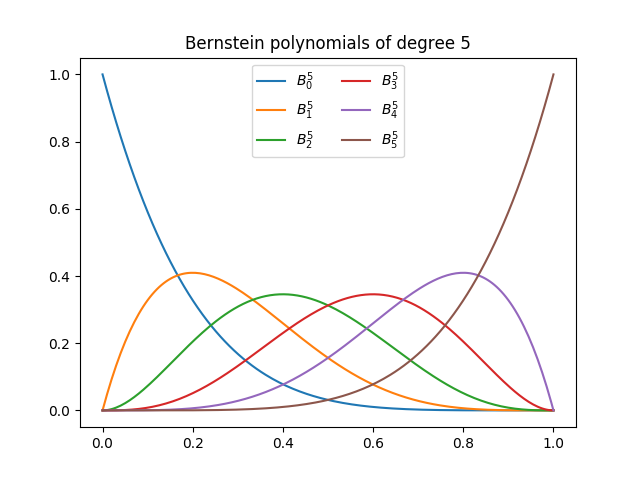
\includegraphics[width=1.0\textwidth]{figures/cad/all_bernstein_degree_5}
\end{minipage}
\caption{Bernstein polynomials of degree $n = 1, 2, 3, 4, 5$.}
  \label{fig:bernstein}
\end{figure}

%%%%%%%%%%%%%%%%%%%%%%
%%  dot2tex bernstein.dot -tmath --figonly > bernstein.tex
%\input{cad/dot/bernstein}
%%%%%%%%%%%%%%%%%%%%%%



\subsubsection*{Properties of Bernstein polynomials}
\begin{itemize}
  \item $B_k^n(x) \ge 0$, for all $k \in \left[0, n \right]$ and $x \in \left[ 0, 1 \right]$ \hfill [positivity] 
  \item $\sum_{k=0}^n B_k^n(x) = 1$, for all $x \in \left[ 0, 1 \right]$ \hfill [partition of unity] 
  \item $B_0^n(0) = B_n^n(1) = 1$ 
  \item $B_k^n$ has exactly one maximum on the interval $\left[ 0, 1 \right]$, at $\frac{k}{n}$ 
  \item $\left( B_k^n(x) \right)_{0 \le k \le n}$ is symmetric with respect to $x = \frac{1}{2}$ \hfill [symmetry]
  \item Bernstein polynomials can be defined recursively using the formulae \ref{eq:bernstein-rec}
    \begin{align}
      B_k^n(x) = (1-x) B_k^{n-1}(x) + x B_{k-1}^{n-1}(x)
      \label{eq:bernstein-rec}
    \end{align}
    where we assume $B_k^n(x) = 0$ is $k < 0$ or $k > n$

    \begin{figure}
    \centering
    \includegraphics[width=0.6\textwidth]{figures/cad/diagrams/bernstein}
    \caption{General evaluation triangular diagram for a Bernstein polynomials.}
    \label{fig:bernstein-triangular-diagram}
    \end{figure}

  \item Bernstein derivatives can be computed using the formulae \ref{eq:bernstein-der} 
    \begin{align}
      {B_k^n}^\prime(x) = n \left(B_{k-1}^{n-1}(x) - B_k^{n-1}(x) \right)
      \label{eq:bernstein-der}
    \end{align}
    using the same assumption as before.
\end{itemize}

%\subsubsection*{Evaluation of Bernstein polynomials}
% TODO move to Jupyter Notebooks
%In this section, we shall see different algorithms to evaluate Bernstein polynomials of a given degree. We first start by the naive implementation given in Code. \ref{code:bernstein_v1}. We see that for every evaluation, we must perform $n$ multiplications to compute the terms in $x$ and $1-x$, while the evaluation of the binomial coefficient takes $n$ multplications and $1$ division. This is clearly not optimal.
%
%\begin{code}
%  \centering
%  \begin{python}
%  from scipy.special import binom
%
%  def bernstein_v1(n,k,x):
%      return binom(n,k) * x**k * (1.-x)**(n-k)
%  \end{python}
%  \caption{Naive implementation for the evaluation of Bernstein polynomials}
%  \label{code:bernstein_v1}
%\end{code}
%
%\begin{code}[ht!]
%\centering
%  \begin{python}
%  def bernstein_v2(n,k,x):
%      if k < 0 or k > n: return 0.
%      if n == 0: return 1.
%      return (1.-x)*bernstein_v2(n-1,k,x) + x*bernstein_v2(n-1,k-1,x)
%  \end{python}
%  \caption{Reccursive implementation for the evaluation of Bernstein polynomials}
%  \label{code:bernstein_v2}
%\end{code}
%
%\begin{code}[ht!]
%\centering
%  \begin{python}
%  from functools import lru_cache
%
%  @lru_cache(maxsize=None)
%  def bernstein_v3(n,k,x):
%      if k < 0 or k > n: return 0.
%      if n == 0: return 1.
%      return (1.-x)*bernstein_v2(n-1,k,x) + x*bernstein_v2(n-1,k-1,x)
%  \end{python}
%  \caption{Reccursive implementation for the evaluation of Bernstein polynomials using \texttt{LRU\_CACHE} decorator in Python, to save all the recent calls.}
%  \label{code:bernstein_v3}
%\end{code}
%
%
%\begin{code}[ht!]
%\centering
%  \begin{python}
%  import numpy as np
%
%  def bernstein_v4(n,k,x):
%      tmp = np.zeros(n+1)
%      tmp[n-k] = 1.
%      x1 = 1.-x
%      for i in range(1, n+1):
%          for j in range(i, n+1)[::-1]:
%              tmp[j] = x1*tmp[j] + x*tmp[j-1]
%      return tmp[n]
%  \end{python}
%  \caption{Naive implementation for the evaluation of Bernstein polynomials}
%  \label{code:bernstein_v4}
%\end{code}
%
%\begin{code}[ht!]
%\centering
%  \begin{python}
%  import numpy as np
%
%  def bernstein_v5(n,k,x,tmp):
%      tmp[:] = 0.
%      tmp[n-k] = 1.
%      x1 = 1.-x
%      for i in range(1, n+1):
%          for j in range(i, n+1)[::-1]:
%              tmp[j] = x1*tmp[j] + x*tmp[j-1]
%      return tmp[n]
%  \end{python}
%  \caption{Naive implementation for the evaluation of Bernstein polynomials}
%  \label{code:bernstein_v5}
%\end{code}
%
%\begin{code}[ht!]
%\centering
%  \begin{python}
%  import numpy as np
%
%  def all_bernstein(n, x):
%      b = np.zeros(n+1)
%      b[0] = 1.
%      x1 = 1.-x
%      for j in range(1, n+1):
%          saved = 0.
%          for i in range(0, j):
%              tmp = b[i]
%              b[i] = saved + x1*tmp
%              saved = x*tmp
%          b[j] = saved
%      return b
%  \end{python}
%  \caption{Evaluation of all Bernstein polynomials}
%  \label{code:all_bernstein}
%\end{code}
%
%
%
%\clearpage
\section{B\'ezier curves}
Rather than taking the power basis as in \ref{eq:power-basis-curve}, Pierre B\'ezier used Bernstein polynomials, in the 1960s while working at \textit{Renault}. This leads to the following definition of a polynomial curve \ref{eq:bezier-curve}

\begin{align}
  \mathcal{C}(t) = \sum_{k=0}^n \mathbf{P}_k B_k^n(t) 
  \label{eq:bezier-curve}
\end{align}
\noindent
The vector coefficients $\left( \mathbf{P} \right)_{0 \le k \le n}$ are called \textit{B\'ezier points} or \textbf{control points}. The reason for this will become clear in the sequel.

\subsubsection*{Examples}
\begin{description}
  \item[\textbf{Example 1.}] A linear ($n=1$) B\'ezier curve (fig. \ref{fig:bezier-ex1}) is defined as 
    $$\mathcal{C}(t) = \mathbf{P}_0 B_0^1(t) + \mathbf{P}_1 B_1^1(t)$$ 
    which describes a straight line from $\mathbf{P}_0$ to $\mathbf{P}_1$, since $B_0^1(t) = 1-t$ and $B_1^1(t) = t$. 

  \begin{figure}
  \centering
  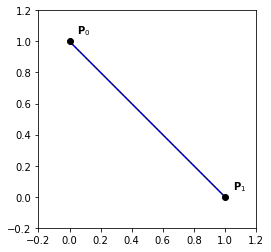
\includegraphics[width=.6\textwidth]{figures/cad/bezier/ex1}
  \caption{Example of a linear B\'ezier curve.}
  \label{fig:bezier-ex1}
  \end{figure}

  \item[\textbf{Example 2.}] A quadratic ($n=2$) B\'ezier curve (fig. \ref{fig:bezier-ex2}) is defined as 
    $$\mathcal{C}(t) = (1-t)^2 \mathbf{P}_0  + 2t(1-t) \mathbf{P}_1 + t^2 \mathbf{P}_2$$  

  \begin{figure}
  \centering
  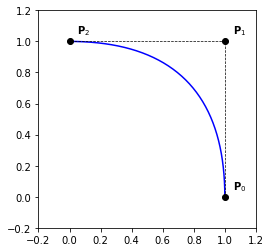
\includegraphics[width=.6\textwidth]{figures/cad/bezier/ex2}
  \caption{Example of a quadratic B\'ezier curve.}
  \label{fig:bezier-ex2}
  \end{figure}

  We remark that
  \begin{itemize}
    \item[-] the curve starts at $\mathbf{P}_{0}$ and  ends at $\mathbf{P}_{2}$,
    \item[-] the curve does not pass through the point $\mathbf{P}_{1}$,
    \item[-] the tangent directions to the curves at its extremeties are parallel to $\mathbf{P}_{1} - \mathbf{P}_{0}$ and $\mathbf{P}_{2} - \mathbf{P}_{1}$,
    \item[-] the curve is contained in the polygone (triangle) formed by $\mathbf{P}_{0}\mathbf{P}_{1}\mathbf{P}_{2}$. This polygone is called the \textit{control polygon} and it approximates the shape of the curve.
  \end{itemize}

  \item[\textbf{Example 3.}] A cubic ($n=3$) B\'ezier curve (figures \ref{fig:bezier-ex3a},\ref{fig:bezier-ex3b},\ref{fig:bezier-ex3c}) is defined as 
    $$\mathcal{C}(t) = (1-t)^3 \mathbf{P}_0  + 3t(1-t)^2 \mathbf{P}_1 + 3t^2(1-t) \mathbf{P}_2 + t^3 \mathbf{P}_3$$  

  \begin{figure}
  \centering
  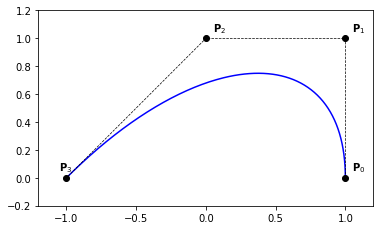
\includegraphics[width=.6\textwidth]{figures/cad/bezier/ex3a}
  \caption{Example of a cubic B\'ezier curve.}
  \label{fig:bezier-ex3a}
  \end{figure}

  \begin{figure}
  \centering
  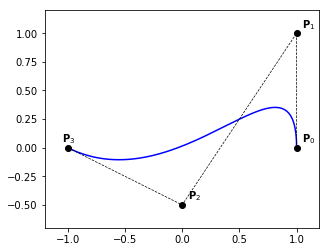
\includegraphics[width=.6\textwidth]{figures/cad/bezier/ex3b}
  \caption{Example of a cubic B\'ezier curve.}
  \label{fig:bezier-ex3b}
  \end{figure}

  \begin{figure}
  \centering
  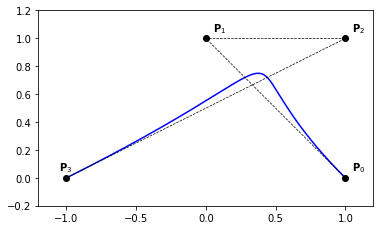
\includegraphics[width=.6\textwidth]{figures/cad/bezier/ex3c}
  \caption{Example of a cubic B\'ezier curve.}
  \label{fig:bezier-ex3c}
  \end{figure}

  We remark that
  \begin{itemize}
    \item[-] the curves start at $\mathbf{P}_{0}$ and end at $\mathbf{P}_{3}$,
    \item[-] the curves do not pass through the points $\mathbf{P}_{1}$ and $\mathbf{P}_{2}$,
    \item[-] the tangents directions to the curves at their extremeties are parallel to $\mathbf{P}_{1} - \mathbf{P}_{0}$ and $\mathbf{P}_{3} - \mathbf{P}_{2}$,
    \item[-] the control polygons approximate the shape of the curves,
    \item[-] the curves follow the orientation of the control polygons,
    \item[-] the curves are contained in the convex hulls of their control polygons (\textit{convex hull property}).
  \end{itemize}

\end{description}


%\begin{figure}[ht!]
%\centering
%\begin{minipage}[t]{1.0\textwidth}
%\begin{python}[caption={TODO},captionpos=b, label={code:point_bezier_curve}]
%def point_on_bezier_curve(P,x):
%    n = len(P) - 1
%    b = all_bernstein(n, x)
%    c = 0.
%    for k in range(0, n+1):
%        c += b[k]*P[k]
%    return c
%\end{python}
%\end{minipage}
%\end{figure}

%\todo{add remarks p22}

\subsubsection*{Derivatives of a B\'ezier curve}
\noindent
Using the formulae \ref{eq:bernstein-der}, we have
\begin{align*}
  \mathcal{C}^\prime(t) = \sum_{k=0}^n \mathbf{P}_k {B_k^n}^\prime(t) 
                        = \sum_{k=0}^n n \mathbf{P}_k \left(B_{k-1}^{n-1}(x) - B_k^{n-1}(x) \right)  
\end{align*}
by reordering the indices, we get \ref{eq:bezier-curve-der}
\begin{align}
  \mathcal{C}^\prime(t) &= \sum_{k=0}^{n-1} n \left( \mathbf{P}_{k+1} - \mathbf{P}_k \right) B_k^{n-1}(t) 
  \label{eq:bezier-curve-der}
\end{align}
Therefor, we get the direct acces to the first order derivatives at the extremeties of a B\'ezier curve using the formulae \ref{eq:bezier-curve-der-1-ext}

\begin{align}
  \begin{cases}
    \mathcal{C}^\prime(0) = n \left( \mathbf{P}_{1} - \mathbf{P}_0 \right)  
    \\ 
    \mathcal{C}^\prime(1) = n \left( \mathbf{P}_{n} - \mathbf{P}_{n-1} \right)  
  \end{cases}
  \label{eq:bezier-curve-der-1-ext}
\end{align}
\noindent
Second derivatives can also be computed directly from the control points using the formulae  \ref{eq:bezier-curve-der-2-ext}

\begin{align}
  \begin{cases}
    \mathcal{C}^{\prime\prime}(0) = n(n-1) \left( \mathbf{P}_{0} - 2 \mathbf{P}_1 + \mathbf{P}_{2} \right)  
    \\ 
    \mathcal{C}^{\prime\prime}(1) = n(n-1) \left( \mathbf{P}_{n} - 2 \mathbf{P}_{n-1} + \mathbf{P}_{n-2} \right)  
  \end{cases}
  \label{eq:bezier-curve-der-2-ext}
\end{align}

%\todo{add formulae for higher derivatives}
%\todo{Explain why the control points are called so}

\begin{definition}[$r^{th}$ forward difference]
  Let us consider a set of (control) points $\mathbf{P}$.
  The $r^{th}$ forward difference of $\mathbf{P}$ is defined as  
  \begin{align*}
    \triangle^r \mathbf{P}_i := \triangle^{r-1} \mathbf{P}_{i+1} - \triangle^{r-1} \mathbf{P}_i  
  \end{align*}
  with 
  \begin{align*}
    \triangle \mathbf{P}_i = \triangle^1 \mathbf{P}_i := \mathbf{P}_{i+1} - \mathbf{P}_i  
  \end{align*}
\end{definition}

\begin{proposition}[High order dirivatives]
  \begin{align}
    \mathcal{C}^{(r)}(t) = \frac{n!}{\left( n-r \right)!} \sum\limits_{i=0}^{n-r} \triangle^r \mathbf{P}_i B_i^{n-r}(t) 
    \label{eq:bezier-high-deriv}
  \end{align}
\end{proposition}
\noindent
Eqs (\ref{eq:bezier-curve-der-1-ext}) and (\ref{eq:bezier-curve-der-2-ext}) can be generelaized for high order derivatives. We have in fact the following result:
\begin{remark}
The derivatives of a B\'ezier curve at its extremeties up to order $r$ depend only on the first (or last) $r+1$ control points, and vice versa.
\end{remark}
\begin{proposition}
  \label{prop:bezier-forward-difference}
  $$\triangle^r \mathbf{P}_0 = \sum\limits_{i=0}^{r} \left( -1 \right)^{r-i} \binom{r}{i} \mathbf{P}_i $$
\end{proposition}

\subsubsection*{Integration of B\'ezier curves}
\begin{proposition}
A primitive of A B\'ezier curve $\mathcal{C}(t) = \sum_{k=0}^n \mathbf{P}_k B_k^n(t)$ has the B\'ezier representation
\begin{align}
  \left( \int \mathcal{C} \right) (t) = \sum_{k=0}^{n+1} \mathbf{Q}_k B_k^{n+1}(t)
  \label{eq:bezier-primitive}
\end{align}
where
\begin{align*}
  \mathbf{Q}_k := \mathbf{Q}_{k-1} + \frac{1}{n+1} \mathbf{P}_{k-1} 
                = \mathbf{Q}_{0}  + \frac{1}{n+1} \left( \sum\limits_{i=0}^{k-1} \mathbf{P}_{i}  \right)
\end{align*}
\end{proposition}
Here, $\mathbf{Q}_{0}$ denotes an arbitrary integration constant.
\begin{remark}
  Using Eq. (\ref{eq:bezier-primitive}), we have $\int_0^1 \mathcal{C}(t)~dt = \frac{1}{n+1}\left( \sum\limits_{i=0}^n \mathbf{P}_i \right)$.
\end{remark}

\subsubsection*{Properties of B\'ezier curves}
Because of the \textit{symmetry} of the Bernstein polynomials, we have
\begin{itemize}
  \item  $\sum_{k=0}^n \mathbf{P}_k B_k^n = \sum_{k=0}^n \mathbf{P}_k B_{n-k}^n $
\end{itemize}
Thanks to the interpolation property, for $B_0^n$ and $B_n^n$, of the Bernstein polynomials at the endpoints, we get
\begin{itemize}
  \item $\mathcal{C}(0) = \mathbf{P}_0$  and $\mathcal{C}(1) = \mathbf{P}_n$ 
\end{itemize}
Using the partition unity property of the Bernstein polynomials, we get
\begin{itemize}
  \item any point $\mathcal{C}(t)$ is an \textit{affine combination} of the control points 
\end{itemize}
Therefor,
\begin{itemize}
  \item B\'ezier curves are affinely invariant; \textit{i.e.} the image curve $\Phi(\sum_{k=0}^n \mathbf{P}_k B_k^n)$ of a B\'ezier curve, by an affine mapping $\Phi$, is the B\'ezier curve having $\left( \Phi(\mathbf{P}_i) \right)_{0 \le i \le n}$ as control points. 
\end{itemize}
due to the partition unity of the Bernstein polynomials and their non-negativity, 
\begin{itemize}
  \item any point $\mathcal{C}(t)$ is a \textit{convex combination} of the control points 
\end{itemize}
finally, we get the \textit{convex hull property},
\begin{itemize}
  \item A B\'ezier curve lies in the convex hull of its control points 
\end{itemize}

\section{DeCasteljau Algorithm}
In this section, we introduce the deCasteljau algorithm Algo. (\ref{algo:decasteljau}). The basic idea comes from the following remark;
using the reccurence formulae Eq. (\ref{eq:bernstein-rec}), we have
\begin{align*}
  \mathcal{C}(t) &= \sum_{k=0}^n \mathbf{P}_k B_k^n(t) = \sum_{k=0}^n \mathbf{P}_k \left( (1-t) B_k^{n-1}(t) + t B_{k-1}^{n-1}(t) \right) \\ 
                 &= \sum_{k=0}^{n-1} \mathbf{P}_k^1  B_k^{n-1}(t) \quad\quad\quad\quad\quad [\mathbf{P}_k^{1} := (1-t)\mathbf{P}_k + t \mathbf{P}_{k+1}] \\ 
                 &= \sum_{k=0}^{n-2} \mathbf{P}_k^2  B_k^{n-2}(t) \quad\quad\quad\quad\quad [\mathbf{P}_k^{2} := (1-t)\mathbf{P}_k^1 + t \mathbf{P}_{k+1}^1] \\ 
                 &= \ldots \\
                 &= \sum_{k=0}^{0} \mathbf{P}_k^n  B_k^{0}(t) \quad\quad\quad\quad\quad [\mathbf{P}_k^{n} := (1-t)\mathbf{P}_k^{n-1} + t \mathbf{P}_{k+1}^{n-1}] \\ 
                 &= \mathbf{P}_0^n 
\end{align*}
% ...
\begin{minipage}{\textwidth}
  \begin{algorithm}[H]
  \DontPrintSemicolon
  \SetAlgoLined
  \SetKwInOut{Input}{Input}\SetKwInOut{Output}{Output}
  \Input{$\mathbf{P}, x$}
  \Output{$value$}
  \BlankLine

  $n \gets {\sc len } \left( \mathbf{P} \right) - 1$\;
  $\mathbf{Q} \gets \mathbf{P}$\;
  \For{$j \gets 0$ \textbf{to} $n$} {
    \For{$i \gets 0$ \textbf{to} $n-j$} {
      $Q[i] \gets (1-x) Q[i] + x Q[i+1]$\;
    }
  }
  \Return{$Q[0]$}\;

  \caption{{\sc DeCasteljau}: Evaluation of a B\'ezier curve, defined by its control points $\mathbf{P}$ at $x$.}
  \label{algo:decasteljau}
  \end{algorithm} 
\end{minipage}
% ...

\section{Conversion from/to monomial form}
\subsubsection*{Conversion from monomial form}
Let us consider a monomial representation of a curve 
\begin{align*}
\mathcal{C}(t) = \sum_{k=0}^n \mathbf{Q}_k t^k 
\end{align*}
Since
\begin{align*}
  t^k &= \frac{1}{\binom{n}{k}} \binom{n}{k} t^k \left(1-t+t \right)^{n-k} 
      = \frac{1}{\binom{n}{k}} \left( \sum\limits_{i=0}^{n-k} \binom{n}{k} \binom{n-k}{n-k-i} t^{i+k} \left( 1-t \right)^{n-k-i} \right) \\
      &= \frac{1}{\binom{n}{k}} \left(  \sum\limits_{i=0}^{n-k} \binom{k+i}{k} B_{k+i}^n(t) \right)
      = \frac{1}{\binom{n}{k}} \left(  \sum\limits_{j=0}^{n} \binom{j}{k} B_{j}^n(t) \right) 
\end{align*}
we get,
\begin{align*}
\mathcal{C}(t) = \sum_{k=0}^n \mathbf{Q}_k t^k = \sum_{k=0}^n \mathbf{Q}_k \frac{1}{\binom{n}{k}} \left(  \sum\limits_{j=0}^{n} \binom{j}{k} B_{j}^n(t) \right)  
\end{align*}
hence,
\begin{align*}
\mathcal{C}(t) = \sum_{j=0}^n \left(\sum\limits_{k=0}^{n} \frac{\binom{j}{k}}{\binom{n}{k}} \mathbf{Q}_k \right) B_{j}^n(t)  
\end{align*}
which is a B\'ezier curve of the form
\begin{align*}
\mathcal{C}(t) = \sum_{k=0}^n \mathbf{P}_k B_k^n(t)
\end{align*}
with 
\begin{align*}
\mathbf{P}_k =  \sum\limits_{k=0}^{n} \frac{\binom{j}{k}}{\binom{n}{k}} \mathbf{Q}_k 
\end{align*}
\begin{remark}
  If $\mathbf{Q}_k = 0$ for all $k \geq 2$, then the control points are given by $\mathbf{P}_k = \mathbf{Q}_0 + k \mathbf{Q}_1$.
\end{remark}
\begin{proposition}[Linear Precision]
  Conversly, if the $n+1$ control points $\mathbf{P}$ lie equidistantly on a line, then $\mathcal{C}$ is a linear polynomial, which can be written as $\mathcal{C}(t) = \left(1-t\right) \mathbf{P}_0 + t \mathbf{P}_n$. 
\end{proposition}
\subsubsection*{Conversion to monomial form}
Given a B\'ezier curve $\mathcal{C}(t) = \sum_{k=0}^n \mathbf{P}_k B_k^n(t)$, we can derive its monomial representation using the Taylor expansion,
\begin{align*}
  \mathcal{C}(t) &= \sum\limits_{k=0}^n \frac{1}{k!}\mathcal{C}^{(k)}(0) t^k \\
                 &= \sum\limits_{k=0}^n \binom{n}{k} \triangle^k \mathbf{P}_0 t^k  
\end{align*}

\section{Rational B\'ezier curves}
We first introduce the notion of Rational Bernstein polynomials defined as,  and $w_i > 0, \forall i \in \left[0, n \right]$ 
\begin{align}
  R_k^n(t) := \frac{w_i B_k^n(t)}{\sum_{i=0}^n w_i B_i^n(t)}
  \label{eq:rational-bernstein}
\end{align}

\subsubsection*{Properties of Rational Bernstein polynomials}
\begin{itemize}
  \item $R_k^n(x) \ge 0$, for all $k \in \left[0, n \right]$ and $x \in \left[ 0, 1 \right]$ \hfill [positivity] 
  \item $\sum_{k=0}^n R_k^n(x) = 1$, for all $x \in \left[ 0, 1 \right]$ \hfill [partition of unity] 
  \item $R_0^n(0) = R_n^n(1) = 1$ 
  \item $R_k^n$ has exactly one maximum on the interval $\left[ 0, 1 \right]$, 
  \item Bernstein polynomials are Rational Bernstein polynomials when all weights are equal
\end{itemize}

\begin{definition}[Rational B\'ezier curve]

\begin{align}
  \mathcal{C}(t) = \sum_{k=0}^n \mathbf{P}_k R_k^n(t) 
  \label{eq:bezier-curve}
\end{align}

where $R_k^n(t) := \frac{w_i B_k^n(t)}{\sum_{i=0}^n w_i B_i^n(t)}$ and $w_i > 0, \forall i \in \left[0, n \right]$ 
  
\end{definition}

\subsubsection*{Examples}
\begin{description}
  \item[\textbf{Example 1.}] We consider the quadratic Rational B\'ezier curve, 

    \begin{figure}
    \centering
    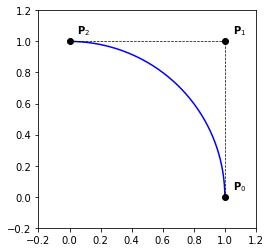
\includegraphics[width=.6\textwidth]{figures/cad/bezier/rational_ex1}
    \caption{Circular arc using quadratic Rational B\'ezier curve.}
    \label{fig:bezier-rational-ex1}
    \end{figure}

    where the weights are given by $w_0 = 1$, $w_1=1$ and $w_2=2$ and the control points are 
    $\mathbf{P}_0 = \begin{pmatrix} 1 \\ 0 \end{pmatrix}$,
    $\mathbf{P}_1 = \begin{pmatrix} 1 \\ 1 \end{pmatrix}$ and
    $\mathbf{P}_2 = \begin{pmatrix} 0 \\ 1 \end{pmatrix}$.
    \\
    This leads to a representation of the circular arc, using the parametric form $\mathcal{C}(t) = \begin{pmatrix} \frac{1-t^2}{1+t^2} \\ \frac{2t}{1+t^2} \end{pmatrix}$.
\end{description}


\section{Composite B\'ezier curves}
A composite B\'ezier curve is a piecewise B\'ezier curve that is at least continuous at the interpolant control points. An example is given in Fig. \ref{fig:composite-bezier-curve}. The global curve inherit all the nice properties of B\'ezier curves however, it has a major drawback: when moving an interpolant control point, we must ensure that the associated regularity is not broken, unless it is what we want. This means that a good representation of a curve needs to have the locality control through control points, but also the control points must be associated to some given regularity. 
\begin{figure}
  \centering
  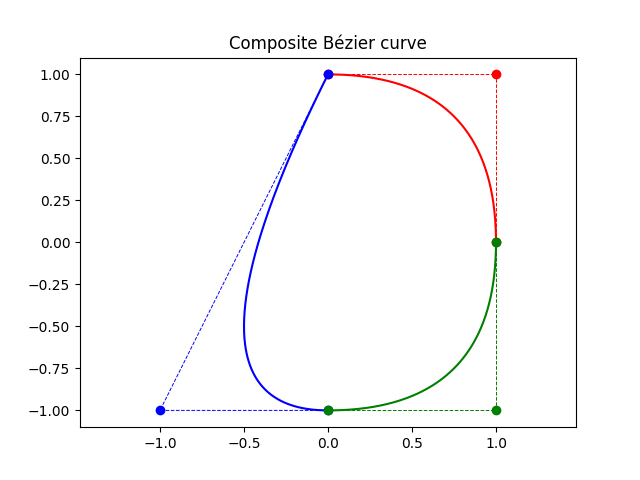
\includegraphics[width=0.6\textwidth]{figures/cad/composite_bezier_curve}
\caption{A composite B\'ezier curve using 3 quadratic B\'ezier curves.}
\label{fig:composite-bezier-curve}
\end{figure}
\noindent
Since Bernstein polynomials are defined locally on the interval $\left[ 0, 1 \right]$, and they do not encode any global redularity of the curve, we need another representation, in terms of other functions, while keeping in mind that these functions must be polynomials on every sub-interval. Such representation is provided by the Schoenberg spaces, for which B-Splines form a basis. In the next chapter, we will first introduce the uniform Splines, also known as Cardinal Splines, show their advantages and limitations, then we will introduce the general definition of B-Splines.



%\section{B\'ezier surfaces}
%\todo{TODO}


%%%%%%%%%%%%%%%%%%%%%%%%%%%%%%%%%%%%%%%%%%%


%\todo{Talk about Gibbs phenomena}

% ...................................................................


\section{Problems}
\label{sec:cad-bezier-problems}

\begin{exercise}
  Show all Bernstein properties.
\end{exercise}

\begin{exercise}
  Consider a cubic B\'ezier curve $\mathcal{C}$ in $\mathbb{R}^2$ with th following control points:
  \begin{align*}
    \mathbf{P}_0 = \left(0, 6 \right), \quad
    \mathbf{P}_1 = \left(3, 6 \right), \quad
    \mathbf{P}_2 = \left(6, 3 \right), \quad
    \mathbf{P}_3 = \left(6, 0 \right)
  \end{align*}
  Compute the point $\mathcal{C}(\frac{1}{3})$ using the deCasteljau algorithm. Compute the same point by Eqs. (\ref{TODO}) and (\ref{TODO}), meaning, evaluate the basis functions at $u=\frac{1}{3}$ then multiply by the associated control points.
\end{exercise}

\begin{exercise}
  The Bernstein operator $\mathcal{B}$ assigns to a function $f$ on $[0,1]$ the polynomial
  \begin{align*}
    \mathcal{B}[f](t) := \sum\limits_{i=0}^n f(\frac{i}{n}) B_i^n(t)
  \end{align*}
  Show that if $f$ is a polynomial of degree $m \leq n$, then $\mathcal{B}[f]$ is also a polynomial of degree $m$.
\end{exercise}

\begin{exercise}
  Show that a planar cubic B\'ezier curve has a cusp if $\mathbf{P}_3$ lies on the parabola
  \begin{align*}
    t \rightarrow \left( \mathbf{P}_0 + \mathbf{P}_1 - \mathbf{P}_2 \right) B_0^2(t) + \mathbf{P}_1 B_1^2(t) + \mathbf{P}_2 B_2^2(t)    
  \end{align*}
\end{exercise}

\begin{exercise}
  For which choices of $\mathbf{P}_3 $ does a planar cubic B\'ezier curve have a loop?
\end{exercise}

\begin{exercise}
  We consider a B\'ezier curve $\mathcal{C}(t) = \sum_{k=0}^n \mathbf{P}_k B_k^n(t)$. 
  \\
  \begin{enumerate}
    \item  Show that using the definition of Bernstein polynomials, we can write $\mathcal{C}$ as
      \begin{align*}
        \mathcal{C}(t) = \left( 1-t \right)^n \left( \sum\limits_{i=0}^n \mathbf{P}_k \binom{n}{k} \left( \frac{t}{1-t} \right)^k \right)
      \end{align*}
    \item Write a modifier version of Horner algorithm based on the previous formula and compute its arithmetic complexity. 
    \item What happens when $t$ is close to $1$? How to adapt the previous algorithm in this case? 
  \end{enumerate}
\end{exercise}

\begin{exercise}
  .
\end{exercise}

\begin{exercise}
  .
\end{exercise}

\begin{exercise}
  .
\end{exercise}

\begin{exercise}
  .
\end{exercise}

\begin{exercise}
  .
\end{exercise}

\begin{exercise}
  .
\end{exercise}




% *********** historical_notes.tex
\chapter{Historical Notes}
\label{ch:cad-historical-notes}

References: \cite{PieglBook1996}, \cite{DeBoor_Book2001}, \cite{farin2002curves, farin1999nurbs, prautzsch2002bezier,rogers2001introduction,cohen2001geometric}


